% Für Bindekorrektur als optionales Argument "BCORfaktormitmaßeinheit", dann
% sieht auch Option "twoside" vernünftig aus
% Näheres zu "scrartcl" bzw. "scrreprt" und "scrbook" siehe KOMA-Skript Doku
\documentclass[12pt,a4paper,titlepage,headinclude,bibtotoc]{scrartcl}

\usepackage{adjustbox}
%---- Allgemeine Layout Einstellungen ------------------------------------------

% Für Kopf und Fußzeilen, siehe auch KOMA-Skript Doku
\usepackage[komastyle]{scrpage2}
\pagestyle{scrheadings}
\setheadsepline{0.5pt}[\color{black}]
\automark[section]{chapter}


%Einstellungen für Figuren- und Tabellenbeschriftungen
\setkomafont{captionlabel}{\sffamily\bfseries}
\setcapindent{0em}


%---- Weitere Pakete -----------------------------------------------------------
% Die Pakete sind alle in der TeX Live Distribution enthalten. Wichtige Adressen
% www.ctan.org, www.dante.de

% Sprachunterstützung
\usepackage[ngerman]{babel}

% Benutzung von Umlauten direkt im Text
% entweder "latin1" oder "utf8"
\usepackage[utf8]{inputenc}

% Pakete mit Mathesymbolen und zur Beseitigung von Schwächen der Mathe-Umgebung
\usepackage{latexsym,exscale,stmaryrd,amssymb,amsmath}

% Weitere Symbole
\usepackage[nointegrals]{wasysym}
\usepackage{eurosym}

% Anderes Literaturverzeichnisformat
%\usepackage[square,sort&compress]{natbib}

% Für Farbe
\usepackage{color}

% Zur Graphikausgabe
%Beipiel: \includegraphics[width=\textwidth]{grafik.png}
\usepackage{graphicx}

% Text umfließt Graphiken und Tabellen
% Beispiel:
% \begin{wrapfigure}[Zeilenanzahl]{"l" oder "r"}{breite}
%   \centering
%   \includegraphics[width=...]{grafik}
%   \caption{Beschriftung} 
%   \label{fig:grafik}
% \end{wrapfigure}
\usepackage{wrapfig}

% Mehrere Abbildungen nebeneinander
% Beispiel:
% \begin{figure}[htb]
%   \centering
%   \subfigure[Beschriftung 1\label{fig:label1}]
%   {\includegraphics[width=0.49\textwidth]{grafik1}}
%   \hfill
%   \subfigure[Beschriftung 2\label{fig:label2}]
%   {\includegraphics[width=0.49\textwidth]{grafik2}}
%   \caption{Beschriftung allgemein}
%   \label{fig:label-gesamt}
% \end{figure}
\usepackage{subfigure}

% Caption neben Abbildung
% Beispiel:
% \sidecaptionvpos{figure}{"c" oder "t" oder "b"}
% \begin{SCfigure}[rel. Breite (normalerweise = 1)][hbt]
%   \centering
%   \includegraphics[width=0.5\textwidth]{grafik.png}
%   \caption{Beschreibung}
%   \label{fig:}
% \end{SCfigure}
\usepackage{sidecap}

% Befehl für "Entspricht"-Zeichen
\newcommand{\corresponds}{\ensuremath{\mathrel{\widehat{=}}}}
% Befehl für Errorfunction
\newcommand{\erf}[1]{\text{ erf}\ensuremath{\left( #1 \right)}}

%Fußnoten zwingend auf diese Seite setzen
\interfootnotelinepenalty=1000

%Für chemische Formeln (von www.dante.de)
%% Anpassung an LaTeX(2e) von Bernd Raichle
\makeatletter
\DeclareRobustCommand{\chemical}[1]{%
  {\(\m@th
   \edef\resetfontdimens{\noexpand\)%
       \fontdimen16\textfont2=\the\fontdimen16\textfont2
       \fontdimen17\textfont2=\the\fontdimen17\textfont2\relax}%
   \fontdimen16\textfont2=2.7pt \fontdimen17\textfont2=2.7pt
   \mathrm{#1}%
   \resetfontdimens}}
\makeatother

%Honecker-Kasten mit $$\shadowbox{$xxxx$}$$
\usepackage{fancybox}

%SI-Package
\usepackage{siunitx}

%keine Einrückung, wenn Latex doppelte Leerzeile
\parindent0pt

%Bibliography \bibliography{literatur} und \cite{gerthsen}
%\usepackage{cite}
\usepackage{babelbib}
\selectbiblanguage{ngerman}

\begin{document}

\begin{titlepage}
\centering
\textsc{\Large Anfängerpraktikum der Fakultät für
  Physik,\\[1.5ex] Universität Göttingen}

\vspace*{4.2cm}

\rule{\textwidth}{1pt}\\[0.5cm]
{\huge \bfseries
Versuch 14\\[1.5ex]
  Wechselstromwiderstände
  }\\[0.5cm]
\rule{\textwidth}{1pt}

\vspace*{2.5cm}

\begin{Large}
\begin{tabular}{ll}
Praktikant: &  Michael Lohmann\\
 Versuchspartner &  Felix Kurtz\\
 E-Mail: & m.lohmann@stud.uni-goettingen.de\\
 Betreuer: & Björn Klaas\\
 Versuchsdatum: & 08.09.2014\\
\end{tabular}
\end{Large}

\vspace*{0.8cm}

\begin{Large}
\fbox{
  \begin{minipage}[t][2.5cm][t]{6cm} 
Eingegangen am:
  \end{minipage}
}
\end{Large}

\end{titlepage}

\tableofcontents

\newpage

\section{Einleitung}
\label{sec:einleitung}
Wechselströme spielen in der modernen Energieversorgung eine zentrale Rolle.
Um so wichtiger ist es, die Effekte und genauen Eigenschaften von \emph{Wechselstrom-Widerständen} zu kennen.
Auch die Phasenverschiebung von Strom zu Spannung soll in diesem Versuch beobachtet werden.
\section{Theorie}
\label{sec:theorie}
\subsection{Wechselspannungen und -ströme}
Unter einer Wechselspannung versteht man eine Spannung, die einen periodischen zeitlichen Verlauf besitzt.
Die zumeist verwendete ist die sinusförmige mit 
\begin{align*}
U(t)=U_0\cdot\sin(\omega t)\quad .
\end{align*}
Da hierbei die maximale Spannung $U_0$ nur den kürzesten Teil der Zeit anliegt, ist die Definition eines \emph{Effektivwertes} sinnvoll.
Diese ist so definiert, dass eine Gleichspannung diesen Wertes die selbe Leistung erbringt, nämlich:
\begin{align*}
U_\text{eff}=\frac{U_0}{\sqrt2}\quad .
\end{align*}
Die in europäischen Haushalten übliche Wechselspannung von $U_\text{eff}=220\,\si\volt$ besitzt so eine Maximalspannung von $U_0=\sqrt2\cdot U_\text{eff}=311\,\si\volt$.
Ebenso ist auch der Effektivstrom definiert.\\

Der fließende Strom $I$ besitzt nun die Form
\begin{align*}
I=I_0\cdot\sin(\omega t+\varphi)
\end{align*}
wobei $\varphi$ die Phasenverschiebung ist.
Diese hängt ab von der jeweiligen Schaltung ab und wird in den Kapiteln \ref{sec:RLC} und \ref{sec:LC} behandelt.

\subsection{Impedanz}
\label{sec:impedanz}
\begin{figure}[!h]
\centering
\input{zeiger.pdf_tex}
\caption{Zeigerdiagramm, welches die Realteile der Spannung gegen ihren Imaginärteil in einer Serienschaltung aufträgt.}
\label{fig:zeiger}
\end{figure}
Die Impedanz $Z$ berechnet sich nach \cite[S. 236]{nolting3} im Allgemeinen durch
\begin{align*}
Z=\frac{U(t)}{I(t)}\quad .
\end{align*}
Dies ist analog zum Ohmschen Widerstand $R=\frac{U}{I}$, wodurch sich der Name Scheinwiderstand $|Z|$ für ihren Betrag ergibt.

In Abb. \ref{fig:zeiger} ist ein Beispiel aufgetragen, in dem man die verschiedenen (Blind-)Widerstände einer Schaltung erkennen kann, die an den einzelnen Bauteilen vorhanden sind.
Im Resonanzfall ist $X_L=X_C$, wodurch die gesammte Impedanz $Z$ real wird und die Phasenverschiebung $\varphi=0$ verschwindet.

Die Phasenverschiebung ist nach \cite[S. 236]{nolting3} definiert als
\begin{align}
\varphi=\arctan\frac{\Im(Z)}{\Re(Z)}\quad .
\end{align}

\subsection{Ohmscher Widerstand}
Für einen Ohmschen Widerstand gilt 
\begin{align*}
U(t)=R\cdot I(t)\quad .
\end{align*}
Strom und Spannung sind also in Phase.
\subsection{Induktivität}
Nach \cite[S. 313]{griffith} gilt für eine Spule
\begin{align}
U_\text{Ind}=-U_L=-L\frac{dI}{dt}\quad .
\end{align}
Hierbei bezeichnet $L$ die Induktivität, welche von der Spulengeometrie abhängt.
Nimmt man nun wieder die Sinus-Spannung an, so folgt:
\begin{align*}
U_0\cdot\sin(\omega t)&=L\frac{dI}{dt}\\
\Rightarrow I(t)&=U_0\frac{1}{\omega L}\cos(\omega t)\quad .
\end{align*}
Dies bedeutet, dass die Spannung dem Strom für eine Schaltung, welche nur aus einer Spule bestehent, um $\varphi=\frac{\pi}{2}$ voraus eilt.

Man kann nun den \emph{Blindwiderstand} für eine Spule definieren:
\begin{align}
X_L:=\frac{U(t)}{I(t)}=L\omega\quad .
\end{align}



\subsection{Kapazität}
Für einen Kondensator gilt nach \cite[S. 822]{giancoli}:
\begin{align*}
Q&=CU=CU_0\sin(\omega t)\\
\Rightarrow I(t)&=\dot Q=CU_0\omega\cos(\omega t)\quad .
\end{align*}
Dies bedeutet, dass der Strom der Spannung um $\varphi=\frac{\pi}{2}$ voraus eilt.

Auch für einen Kondensator kann man so einen \emph{Blindwiederstand} definieren:
\begin{align}
X_C:=\frac{U(t)}{I(t)}=-\frac{1}{\omega C}
\end{align}

\subsection{$RLC$-Serienschaltung}
\label{sec:RLC}
Ein $RLC$-Serienschaltkreis wie in Abb. \ref{fig:serienschaltung} muss nun aus einer Zusammensetzung der beiden erfolgen.
Dafür definiert man die \emph{Impedanz}:
\begin{align}
|Z_\text{Serie}|=\left|R+i(X_L+X_C)\right|=\left|R+i\left( \omega L-\frac{1}{\omega C} \right)\right|=\sqrt{R^2+(X_L+X_C)^2}\quad .
\label{eq:ZSerie}
\end{align}
Die Phasenverschiebung lässt sich (wie in Abb. \ref{fig:zeiger} zu erkennen und nach \cite[S. 1042]{giancoli}) durch
\begin{align}
\varphi=\arctan\left( \frac{X_L+X_C}{R} \right)
\label{eq:PhaseSerie}
\end{align}
berechnen.

\subsection{$LC$-Parallelschaltung}
\label{sec:LC}
Ist ein $LC$-Parallelschaltkreis wie in Abb. \ref{fig:parallel} vorhanden, so berechnet sich die Impedanz nach der Spannungsregel für Parallelkreise durch
\begin{align}
Z_{||}=\frac{-i}{\frac{1}{X_L}+\frac{1}{X_C}}=\left( \frac{1}{R_L+i\omega L}+i\omega C \right)^{-1}
\end{align}
und dem Blindwiderstand
\begin{align}
|Z|=\left[\left(\omega C - \frac{\omega L}{R_L^2+(\omega L)^2}\right)^2+\left(\frac{R_L}{R_L^2+(\omega L)^2}\right)^2\right]^{-\frac{1}{2}}\label{eq:ZPara}\quad .
\end{align}
\section{Durchführung}
\label{sec:durchfuehrung}
Der Aufbau besteht aus einem Frequenzgenerator, welcher einem veränderlichen Stromkreis aus Widerstand, Kondensator und Luftspule Spannung bereitstellt.
Die verschiedenen Parameter Ausgangsspannung $U$, Spannung an Widerstand und Spule $U_{L+R}$, Spannung am Kondensator $U_C$ und Gesamtstrom $I$ werden mit einem Oszilloskop bzw. Spannungs- und Strom-Messgeräten vermessen.\\

\begin{figure}[!h]
\centering
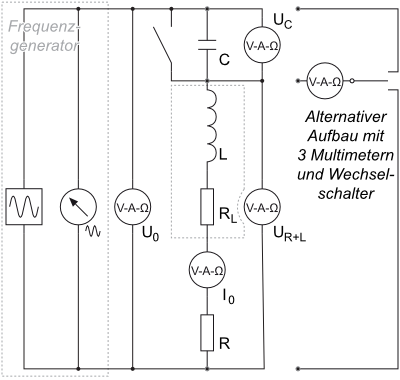
\includegraphics[width=0.5\linewidth]{serie}
\caption{Schaltplan der Serienschaltung nach \cite[4.10.2014, 15:30]{LP14}.}
\label{fig:serienschaltung}
\end{figure}
Zunächst baut man den Serienschaltkreis aus Abb. \ref{fig:serienschaltung} auf.

Dabei wird der Kondensator zunächst überbrückt und erst nach 10 Messungen mit verschiedenen Frequenzen, bei denen Strom $I$ und Spannung $U$ protokolliert werden, hinzugeschaltet.
Alle gemessenen Parameter sollen nun für möglichst viele verschiedene Frequenzen $f$ aufgezeichnet werden.
Mit aktivem Kondensator müssen zusätzlich noch $U_C$ und $U_{R+L}$ sowie die Phasenverschiebung $\varphi$ notiert werden.
Das Oszilloskop wird zur Bestimmung dieser einerseits zur Vermessung der Ausgangsspannung $U$ und andererseits zum Bestimmen des Stroms mit einer Stromzange verwendet.
Bei der Nutzung der Stromzange ist darauf zu achten, dass sich in der Nähe keine anderen Magnetfelder oder stromdurchflossenen Kabel befinden, da dies die Messung stark verfälschen würde.
Es kann nun die beiden Kurven mit Hilfe des Mathe-Modus direkt auf deren Phasenverschiebung hin auswerten.
Damit dies zuverlässig geschieht, ist darauf zu achten, dass die jeweiligen $y$-Achsen so gewählt sind, dass die Kurven ungefähr die selben Ausschläge zeigen.
Auch muss mehr als eine Periode angezeigt werden.
Dabei ist der Resonanzbereich besonders genau zu untersuchen.\\

\begin{figure}[!h]
\centering
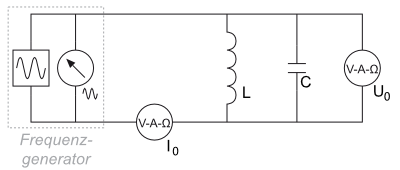
\includegraphics[width=0.6\linewidth]{parallel}
\caption{Schaltplan der Parallelschaltung von \cite[4.10.2014, 15:30]{LP14}.}
\label{fig:parallel}
\end{figure}
Im zweiten Versuchsteil soll ein Parallelkreis aus Kondensator und Spule vermessen werden.
In dieser Messung sollen die Spannung $U$ und der Gesamtstrom $I$ für verschiedene Frequenzen ausgewertet werden.
Auch hier soll die Resonanzstelle wieder besonders genau untersucht werden.\\

Für die Auswertung werden abschließend die Daten der einzelnen Bauteile aufgezeichnet.
Dies sind:
\begin{itemize}
\item Einzelner ohmscher Widerstand $R_\Omega$
\item Ohmscher Widerstand der Spule $R_L$
\item Innenwiderstand des Amperemeters $R_A$
\item Kapazität des Kondensators $C$.
\end{itemize}

Während der Messungen ist darauf zu achten, dass die hier verwendeten Spannungen \emph{tödlich} sein können und dass deshalb auf keinen Fall blanke Kabelenden herumliegen dürfen.
Auch muss vor jeder Änderung am Aufbau sichergestellt werden, dass die Spannung abgeschaltet ist.

\newpage
\section{Auswertung}
\label{sec:auswertung}
\subsection{Widerstand und Spule in Reihe}
\begin{figure}[!htb]
	\centering
	\input{messung1.tex}
	\caption{Quadrat des Scheinwiderstands als Funktion der Kreisfrequenz.}
	\label{fig:messung1}
\end{figure}
Da zu Beginn der Kondensator überbrückt ist, ergibt sich aus der quadrierten Gleichung \eqref{eq:ZSerie} nur
\begin{align*}
Z^2=R^2+\omega^2L^2\quad .
\end{align*}
Trägt man also $\omega^2$ gegen $Z^2$ auf, so ergibt sich eine Gerade $y=mx+b$ mit $b=R^2$ und $m=L^2$
Aus dem Fit der Abb. \ref{fig:messung1} ergibt sich so:
\begin{align*}
	L&=(386.3\pm 0.6)\,\si{\milli\henry}\quad \text{und}\\
	R_\text{ges}&=(77.3 \pm 1.1)\,\si{\ohm}\quad .
\end{align*}
\subsection{$RLC$-Serienschaltung}
\begin{figure}[!htb]
	\centering
	% GNUPLOT: LaTeX picture with Postscript
\begingroup
  \makeatletter
  \providecommand\color[2][]{%
    \GenericError{(gnuplot) \space\space\space\@spaces}{%
      Package color not loaded in conjunction with
      terminal option `colourtext'%
    }{See the gnuplot documentation for explanation.%
    }{Either use 'blacktext' in gnuplot or load the package
      color.sty in LaTeX.}%
    \renewcommand\color[2][]{}%
  }%
  \providecommand\includegraphics[2][]{%
    \GenericError{(gnuplot) \space\space\space\@spaces}{%
      Package graphicx or graphics not loaded%
    }{See the gnuplot documentation for explanation.%
    }{The gnuplot epslatex terminal needs graphicx.sty or graphics.sty.}%
    \renewcommand\includegraphics[2][]{}%
  }%
  \providecommand\rotatebox[2]{#2}%
  \@ifundefined{ifGPcolor}{%
    \newif\ifGPcolor
    \GPcolortrue
  }{}%
  \@ifundefined{ifGPblacktext}{%
    \newif\ifGPblacktext
    \GPblacktexttrue
  }{}%
  % define a \g@addto@macro without @ in the name:
  \let\gplgaddtomacro\g@addto@macro
  % define empty templates for all commands taking text:
  \gdef\gplbacktext{}%
  \gdef\gplfronttext{}%
  \makeatother
  \ifGPblacktext
    % no textcolor at all
    \def\colorrgb#1{}%
    \def\colorgray#1{}%
  \else
    % gray or color?
    \ifGPcolor
      \def\colorrgb#1{\color[rgb]{#1}}%
      \def\colorgray#1{\color[gray]{#1}}%
      \expandafter\def\csname LTw\endcsname{\color{white}}%
      \expandafter\def\csname LTb\endcsname{\color{black}}%
      \expandafter\def\csname LTa\endcsname{\color{black}}%
      \expandafter\def\csname LT0\endcsname{\color[rgb]{1,0,0}}%
      \expandafter\def\csname LT1\endcsname{\color[rgb]{0,1,0}}%
      \expandafter\def\csname LT2\endcsname{\color[rgb]{0,0,1}}%
      \expandafter\def\csname LT3\endcsname{\color[rgb]{1,0,1}}%
      \expandafter\def\csname LT4\endcsname{\color[rgb]{0,1,1}}%
      \expandafter\def\csname LT5\endcsname{\color[rgb]{1,1,0}}%
      \expandafter\def\csname LT6\endcsname{\color[rgb]{0,0,0}}%
      \expandafter\def\csname LT7\endcsname{\color[rgb]{1,0.3,0}}%
      \expandafter\def\csname LT8\endcsname{\color[rgb]{0.5,0.5,0.5}}%
    \else
      % gray
      \def\colorrgb#1{\color{black}}%
      \def\colorgray#1{\color[gray]{#1}}%
      \expandafter\def\csname LTw\endcsname{\color{white}}%
      \expandafter\def\csname LTb\endcsname{\color{black}}%
      \expandafter\def\csname LTa\endcsname{\color{black}}%
      \expandafter\def\csname LT0\endcsname{\color{black}}%
      \expandafter\def\csname LT1\endcsname{\color{black}}%
      \expandafter\def\csname LT2\endcsname{\color{black}}%
      \expandafter\def\csname LT3\endcsname{\color{black}}%
      \expandafter\def\csname LT4\endcsname{\color{black}}%
      \expandafter\def\csname LT5\endcsname{\color{black}}%
      \expandafter\def\csname LT6\endcsname{\color{black}}%
      \expandafter\def\csname LT7\endcsname{\color{black}}%
      \expandafter\def\csname LT8\endcsname{\color{black}}%
    \fi
  \fi
  \setlength{\unitlength}{0.0500bp}%
  \begin{picture}(7200.00,5040.00)%
    \gplgaddtomacro\gplbacktext{%
      \csname LTb\endcsname%
      \put(946,704){\makebox(0,0)[r]{\strut{} 0}}%
      \put(946,1156){\makebox(0,0)[r]{\strut{} 0.2}}%
      \put(946,1609){\makebox(0,0)[r]{\strut{} 0.4}}%
      \put(946,2061){\makebox(0,0)[r]{\strut{} 0.6}}%
      \put(946,2513){\makebox(0,0)[r]{\strut{} 0.8}}%
      \put(946,2966){\makebox(0,0)[r]{\strut{} 1}}%
      \put(946,3418){\makebox(0,0)[r]{\strut{} 1.2}}%
      \put(946,3870){\makebox(0,0)[r]{\strut{} 1.4}}%
      \put(946,4323){\makebox(0,0)[r]{\strut{} 1.6}}%
      \put(946,4775){\makebox(0,0)[r]{\strut{} 1.8}}%
      \put(1078,484){\makebox(0,0){\strut{} 0}}%
      \put(1794,484){\makebox(0,0){\strut{} 0.5}}%
      \put(2509,484){\makebox(0,0){\strut{} 1}}%
      \put(3225,484){\makebox(0,0){\strut{} 1.5}}%
      \put(3941,484){\makebox(0,0){\strut{} 2}}%
      \put(4656,484){\makebox(0,0){\strut{} 2.5}}%
      \put(5372,484){\makebox(0,0){\strut{} 3}}%
      \put(6087,484){\makebox(0,0){\strut{} 3.5}}%
      \put(6803,484){\makebox(0,0){\strut{} 4}}%
      \put(176,2739){\rotatebox{-270}{\makebox(0,0){\strut{}$Z$ [k$\Omega$]}}}%
      \put(3940,154){\makebox(0,0){\strut{}$\omega$ [kHz]}}%
    }%
    \gplgaddtomacro\gplfronttext{%
      \csname LTb\endcsname%
      \put(5816,4602){\makebox(0,0)[r]{\strut{}Messwerte}}%
      \csname LTb\endcsname%
      \put(5816,4382){\makebox(0,0)[r]{\strut{}Fit nach Gl. \eqref{eq:ZSerie}}}%
    }%
    \gplbacktext
    \put(0,0){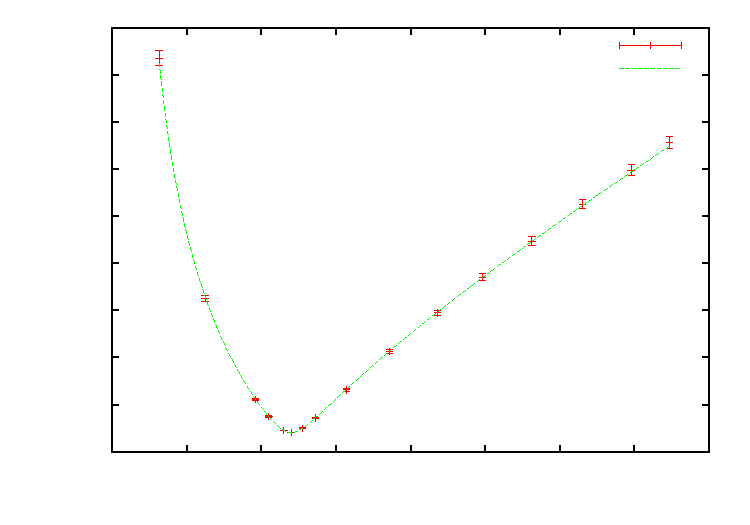
\includegraphics{messung2}}%
    \gplfronttext
  \end{picture}%
\endgroup

	\caption{Scheinwiderstand des Serienresonanzkreis als Funktion der Kreisfrequenz.}
	\label{fig:messung2}
\end{figure}
In Abb. \ref{fig:messung2} wird der Scheinwiderstand gegen die Kreisfrequenz aufgetragen.
Der Fit nach der theoretischen Kurve \eqref{eq:ZSerie} ermittelte so 
\begin{align*}
	R &= (80.9 \pm 0.5)\,\si{\ohm}\quad ,\\
	L &= (386.1 \pm 1.0)\,\si{\milli\henry}\quad \text{und}\\
	C &= (1.799 \pm 0.005)\,\si{\micro\farad}
\end{align*}
als Werte.\\

Die gewichteten Mittelwerte aus den bisherigen Werten betragen:
\begin{align*}
\overline L&=(386.2 \pm 0.6)\si{\milli\henry}\\
\overline R&=(80.3 \pm 0.5)\,\si{\ohm}
\end{align*}
\begin{figure}[!htb]
	\centering
	% GNUPLOT: LaTeX picture with Postscript
\begingroup
  \makeatletter
  \providecommand\color[2][]{%
    \GenericError{(gnuplot) \space\space\space\@spaces}{%
      Package color not loaded in conjunction with
      terminal option `colourtext'%
    }{See the gnuplot documentation for explanation.%
    }{Either use 'blacktext' in gnuplot or load the package
      color.sty in LaTeX.}%
    \renewcommand\color[2][]{}%
  }%
  \providecommand\includegraphics[2][]{%
    \GenericError{(gnuplot) \space\space\space\@spaces}{%
      Package graphicx or graphics not loaded%
    }{See the gnuplot documentation for explanation.%
    }{The gnuplot epslatex terminal needs graphicx.sty or graphics.sty.}%
    \renewcommand\includegraphics[2][]{}%
  }%
  \providecommand\rotatebox[2]{#2}%
  \@ifundefined{ifGPcolor}{%
    \newif\ifGPcolor
    \GPcolortrue
  }{}%
  \@ifundefined{ifGPblacktext}{%
    \newif\ifGPblacktext
    \GPblacktexttrue
  }{}%
  % define a \g@addto@macro without @ in the name:
  \let\gplgaddtomacro\g@addto@macro
  % define empty templates for all commands taking text:
  \gdef\gplbacktext{}%
  \gdef\gplfronttext{}%
  \makeatother
  \ifGPblacktext
    % no textcolor at all
    \def\colorrgb#1{}%
    \def\colorgray#1{}%
  \else
    % gray or color?
    \ifGPcolor
      \def\colorrgb#1{\color[rgb]{#1}}%
      \def\colorgray#1{\color[gray]{#1}}%
      \expandafter\def\csname LTw\endcsname{\color{white}}%
      \expandafter\def\csname LTb\endcsname{\color{black}}%
      \expandafter\def\csname LTa\endcsname{\color{black}}%
      \expandafter\def\csname LT0\endcsname{\color[rgb]{1,0,0}}%
      \expandafter\def\csname LT1\endcsname{\color[rgb]{0,1,0}}%
      \expandafter\def\csname LT2\endcsname{\color[rgb]{0,0,1}}%
      \expandafter\def\csname LT3\endcsname{\color[rgb]{1,0,1}}%
      \expandafter\def\csname LT4\endcsname{\color[rgb]{0,1,1}}%
      \expandafter\def\csname LT5\endcsname{\color[rgb]{1,1,0}}%
      \expandafter\def\csname LT6\endcsname{\color[rgb]{0,0,0}}%
      \expandafter\def\csname LT7\endcsname{\color[rgb]{1,0.3,0}}%
      \expandafter\def\csname LT8\endcsname{\color[rgb]{0.5,0.5,0.5}}%
    \else
      % gray
      \def\colorrgb#1{\color{black}}%
      \def\colorgray#1{\color[gray]{#1}}%
      \expandafter\def\csname LTw\endcsname{\color{white}}%
      \expandafter\def\csname LTb\endcsname{\color{black}}%
      \expandafter\def\csname LTa\endcsname{\color{black}}%
      \expandafter\def\csname LT0\endcsname{\color{black}}%
      \expandafter\def\csname LT1\endcsname{\color{black}}%
      \expandafter\def\csname LT2\endcsname{\color{black}}%
      \expandafter\def\csname LT3\endcsname{\color{black}}%
      \expandafter\def\csname LT4\endcsname{\color{black}}%
      \expandafter\def\csname LT5\endcsname{\color{black}}%
      \expandafter\def\csname LT6\endcsname{\color{black}}%
      \expandafter\def\csname LT7\endcsname{\color{black}}%
      \expandafter\def\csname LT8\endcsname{\color{black}}%
    \fi
  \fi
  \setlength{\unitlength}{0.0500bp}%
  \begin{picture}(7200.00,5040.00)%
    \gplgaddtomacro\gplbacktext{%
      \csname LTb\endcsname%
      \put(946,704){\makebox(0,0)[r]{\strut{}-2}}%
      \put(946,1213){\makebox(0,0)[r]{\strut{}-1.5}}%
      \put(946,1722){\makebox(0,0)[r]{\strut{}-1}}%
      \put(946,2231){\makebox(0,0)[r]{\strut{}-0.5}}%
      \put(946,2740){\makebox(0,0)[r]{\strut{} 0}}%
      \put(946,3248){\makebox(0,0)[r]{\strut{} 0.5}}%
      \put(946,3757){\makebox(0,0)[r]{\strut{} 1}}%
      \put(946,4266){\makebox(0,0)[r]{\strut{} 1.5}}%
      \put(946,4775){\makebox(0,0)[r]{\strut{} 2}}%
      \put(1078,484){\makebox(0,0){\strut{} 0}}%
      \put(1794,484){\makebox(0,0){\strut{} 0.5}}%
      \put(2509,484){\makebox(0,0){\strut{} 1}}%
      \put(3225,484){\makebox(0,0){\strut{} 1.5}}%
      \put(3941,484){\makebox(0,0){\strut{} 2}}%
      \put(4656,484){\makebox(0,0){\strut{} 2.5}}%
      \put(5372,484){\makebox(0,0){\strut{} 3}}%
      \put(6087,484){\makebox(0,0){\strut{} 3.5}}%
      \put(6803,484){\makebox(0,0){\strut{} 4}}%
      \put(176,2739){\rotatebox{-270}{\makebox(0,0){\strut{}$\varphi$ [rad]}}}%
      \put(3940,154){\makebox(0,0){\strut{}$\omega$ [kHz]}}%
    }%
    \gplgaddtomacro\gplfronttext{%
      \csname LTb\endcsname%
      \put(5816,1317){\makebox(0,0)[r]{\strut{}Messwerte}}%
      \csname LTb\endcsname%
      \put(5816,1097){\makebox(0,0)[r]{\strut{}linearer Fit um $\omega_R$}}%
      \csname LTb\endcsname%
      \put(5816,877){\makebox(0,0)[r]{\strut{}Fit nach Gl. \eqref{eq:PhaseSerie}, $R=80.3\,\si{\ohm}$}}%
    }%
    \gplbacktext
    \put(0,0){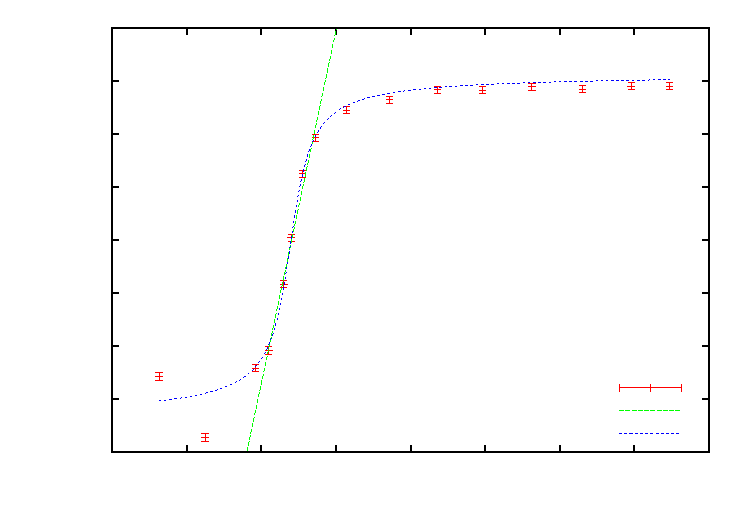
\includegraphics{phase}}%
    \gplfronttext
  \end{picture}%
\endgroup

	\caption{Phasenverschiebung des Serienresonanzkreises.}
	\label{fig:phase}
\end{figure}
Nach \cite[S. 954]{tipler} gilt: 
\begin{align*}
\omega_{R\text{ LC}}&=\frac{1}{\sqrt{LC}}\quad \text{mit}\\
\sigma_{\omega_{R\text{ LC}}}&=\frac{\sqrt{\frac{\sigma_{L}^{2}}{L^{2}} + \frac{\sigma_{C}^{2}}{C^{2}}}}{2 \cdot \sqrt{CL}}\\
\omega_{R\text{ LC}}&=(1199.9 \pm 2.3)\,\si{\hertz}
\end{align*}
wobei die Werte aus dem Fit von Abb. \ref{fig:messung2} stammen.
Aus dem Fit nach Gleichung \eqref{eq:PhaseSerie} von Abb. \ref{fig:phase} kann man $L$ und $C$ bestimmen.
Dies ist möglich, da für $R=80.3\,\si\ohm$ der Mittelwert der vorigen Messungen verwendet wurde.
Es ergeben sich:
\begin{align*}
C&= (1.80 \pm 0.23)\,\si{\micro\farad}\quad\text{und}\\ 
L&= (390\pm 50)\,\si{\milli\henry}\quad .
\end{align*}
Da um die Resonanzfrequenz $\omega_R$ der Arcustangens ungefähr linear ist, lässt sich in diesem Bereich eine Gerade $y=m\cdot x+b$ an die Messwerte fitten, für die gilt:
\begin{align*}
\omega_\text{Phase}&=- \frac{b}{m}\\
\sigma_{\omega_\text{Phase}}&=\frac{1}{m^{2}} \cdot \sqrt{b^{2} \cdot \sigma_{m}^{2} + m^{2} \cdot \sigma_{b}^{2}}\\
\omega_\text{Phase}&=(1200 \pm 120)\,\si\hertz
\end{align*}
\subsubsection{Teilspannungen}
\begin{figure}[!htb]
	\centering
	\input{spannungen.tex}
	\caption{Teilspannungen des Serienresonanzkreises.}
	\label{fig:teilU}
\end{figure}
In Abb. \ref{fig:teilU} sind die Teilspannungen $U_C$ und $U_{L+R}$ in Abhängigkeit der Frequenz aufgetragen.
Dabei fällt auf, dass beide ihr Maximum bei der Resonanzfrequenz haben.
Außerdem sind diese hier ungefähr gleich groß, wie schon in Kapitel \ref{sec:impedanz} erwähnt.
In der Abbildung \ref{fig:zeigerU} sind die Spannungen $U_C$ und $U_{L+R}$ sowie die Gesamtspannung $U$ maßstabsgetreu eingezeichnet, welche sich bei der Messung der Resonanzfrequenz ergeben.
Dazu werden die Messwerte bei einer gemessenen Phasenverschiebung von $1\si\degree$ verwendet: $U=9.26\,$V, $U_C=52.9\,$V und $U_{L+R}=53.4\,$V. 
Der eingezeichnete Winkel $\varphi=\arccos\left(\frac{U}{U_{L+R}}\right)=80\si\degree=1.396\,$rad ist die Phasenverschiebung zwischen $U_{L+R}$ und dem Strom $I$.
Da hier kein kapazitiver Widerstand vorhanden ist, kann man diese Verschiebung auch mit der Formel \eqref{eq:PhaseSerie} ausrechnen. Dazu wird $C=0$ gesetzt:
\begin{align*}
	\varphi=\arctan\left(\frac{\omega_R L}{R}\right)\,.
\end{align*}
Da alle drei Größen fehlerbehaftet sind, folgt mit der Gauss'schen Fehlerfortpflanzung
\begin{align*}	
	\sigma_{\varphi}=\frac{1}{(L \omega_R)^{2} + R^{2}} \cdot \sqrt{(LR)^{2}\, \sigma_{\omega_R}^{2} + (L \omega_R)^{2}\,\sigma_{R}^{2}  + (R \omega_R)^{2}\,\sigma_{L}^{2}}\,.
\end{align*}
Für die gewichteten Mittelwerte $\overline{\omega_R}=(1199.9\pm 2.3)\,\si\hertz$, $\overline{R}=(80.3 \pm 0.5)\,\si\ohm$ und $\overline{L}=(386.2 \pm 0.6)\,\si{\milli\henry}$ ergibt sich eine Phasenverschiebung von
\begin{align*}
	\varphi=(1.399 \pm 0.001)\,\si{rad}\quad.
\end{align*}

\begin{figure}
	\centering	
	\adjustbox{height=0.4\textheight}{\input{SpannungenZeiger.pdf_tex}}
	\caption{Zeigerdiagramm der Spannungen $U$, $U_C$ und $U_{L+R}$ der Serienschaltung bei der Resonanzfrequenz $\omega_R$}
	\label{fig:zeigerU}
\end{figure}
\subsection{Parallelkreis}
In Abb. \ref{fig:messung3} ist der Scheinwiderstand $Z$ gegen die Kreisfrequenz für den Parallelkreis aufgetragen.
Aus dem Fit nach Formel \eqref{eq:ZPara} dieser Abbildung ergibt sich
\begin{align*}
R &= (68\pm 5)\si{\kilo\ohm}\quad ,\\
L &= (370 \pm 10)\si{\milli\henry}\quad \text{und}\\
C &= (1.88  \pm 0.05) \si{\micro\farad}\quad .
\end{align*}
\begin{figure}[!htb]
	\centering
	% GNUPLOT: LaTeX picture with Postscript
\begingroup
  \makeatletter
  \providecommand\color[2][]{%
    \GenericError{(gnuplot) \space\space\space\@spaces}{%
      Package color not loaded in conjunction with
      terminal option `colourtext'%
    }{See the gnuplot documentation for explanation.%
    }{Either use 'blacktext' in gnuplot or load the package
      color.sty in LaTeX.}%
    \renewcommand\color[2][]{}%
  }%
  \providecommand\includegraphics[2][]{%
    \GenericError{(gnuplot) \space\space\space\@spaces}{%
      Package graphicx or graphics not loaded%
    }{See the gnuplot documentation for explanation.%
    }{The gnuplot epslatex terminal needs graphicx.sty or graphics.sty.}%
    \renewcommand\includegraphics[2][]{}%
  }%
  \providecommand\rotatebox[2]{#2}%
  \@ifundefined{ifGPcolor}{%
    \newif\ifGPcolor
    \GPcolortrue
  }{}%
  \@ifundefined{ifGPblacktext}{%
    \newif\ifGPblacktext
    \GPblacktexttrue
  }{}%
  % define a \g@addto@macro without @ in the name:
  \let\gplgaddtomacro\g@addto@macro
  % define empty templates for all commands taking text:
  \gdef\gplbacktext{}%
  \gdef\gplfronttext{}%
  \makeatother
  \ifGPblacktext
    % no textcolor at all
    \def\colorrgb#1{}%
    \def\colorgray#1{}%
  \else
    % gray or color?
    \ifGPcolor
      \def\colorrgb#1{\color[rgb]{#1}}%
      \def\colorgray#1{\color[gray]{#1}}%
      \expandafter\def\csname LTw\endcsname{\color{white}}%
      \expandafter\def\csname LTb\endcsname{\color{black}}%
      \expandafter\def\csname LTa\endcsname{\color{black}}%
      \expandafter\def\csname LT0\endcsname{\color[rgb]{1,0,0}}%
      \expandafter\def\csname LT1\endcsname{\color[rgb]{0,1,0}}%
      \expandafter\def\csname LT2\endcsname{\color[rgb]{0,0,1}}%
      \expandafter\def\csname LT3\endcsname{\color[rgb]{1,0,1}}%
      \expandafter\def\csname LT4\endcsname{\color[rgb]{0,1,1}}%
      \expandafter\def\csname LT5\endcsname{\color[rgb]{1,1,0}}%
      \expandafter\def\csname LT6\endcsname{\color[rgb]{0,0,0}}%
      \expandafter\def\csname LT7\endcsname{\color[rgb]{1,0.3,0}}%
      \expandafter\def\csname LT8\endcsname{\color[rgb]{0.5,0.5,0.5}}%
    \else
      % gray
      \def\colorrgb#1{\color{black}}%
      \def\colorgray#1{\color[gray]{#1}}%
      \expandafter\def\csname LTw\endcsname{\color{white}}%
      \expandafter\def\csname LTb\endcsname{\color{black}}%
      \expandafter\def\csname LTa\endcsname{\color{black}}%
      \expandafter\def\csname LT0\endcsname{\color{black}}%
      \expandafter\def\csname LT1\endcsname{\color{black}}%
      \expandafter\def\csname LT2\endcsname{\color{black}}%
      \expandafter\def\csname LT3\endcsname{\color{black}}%
      \expandafter\def\csname LT4\endcsname{\color{black}}%
      \expandafter\def\csname LT5\endcsname{\color{black}}%
      \expandafter\def\csname LT6\endcsname{\color{black}}%
      \expandafter\def\csname LT7\endcsname{\color{black}}%
      \expandafter\def\csname LT8\endcsname{\color{black}}%
    \fi
  \fi
  \setlength{\unitlength}{0.0500bp}%
  \begin{picture}(7200.00,5040.00)%
    \gplgaddtomacro\gplbacktext{%
      \csname LTb\endcsname%
      \put(946,704){\makebox(0,0)[r]{\strut{} 0}}%
      \put(946,1383){\makebox(0,0)[r]{\strut{} 0.5}}%
      \put(946,2061){\makebox(0,0)[r]{\strut{} 1}}%
      \put(946,2740){\makebox(0,0)[r]{\strut{} 1.5}}%
      \put(946,3418){\makebox(0,0)[r]{\strut{} 2}}%
      \put(946,4097){\makebox(0,0)[r]{\strut{} 2.5}}%
      \put(946,4775){\makebox(0,0)[r]{\strut{} 3}}%
      \put(1078,484){\makebox(0,0){\strut{} 0}}%
      \put(1794,484){\makebox(0,0){\strut{} 0.5}}%
      \put(2509,484){\makebox(0,0){\strut{} 1}}%
      \put(3225,484){\makebox(0,0){\strut{} 1.5}}%
      \put(3941,484){\makebox(0,0){\strut{} 2}}%
      \put(4656,484){\makebox(0,0){\strut{} 2.5}}%
      \put(5372,484){\makebox(0,0){\strut{} 3}}%
      \put(6087,484){\makebox(0,0){\strut{} 3.5}}%
      \put(6803,484){\makebox(0,0){\strut{} 4}}%
      \put(176,2739){\rotatebox{-270}{\makebox(0,0){\strut{}$Z$ [k$\Omega$]}}}%
      \put(3940,154){\makebox(0,0){\strut{}$\omega$ [kHz]}}%
    }%
    \gplgaddtomacro\gplfronttext{%
      \csname LTb\endcsname%
      \put(5816,4602){\makebox(0,0)[r]{\strut{}Messwerte}}%
      \csname LTb\endcsname%
      \put(5816,4382){\makebox(0,0)[r]{\strut{}Fit nach Gl. \eqref{eq:ZPara}}}%
    }%
    \gplbacktext
    \put(0,0){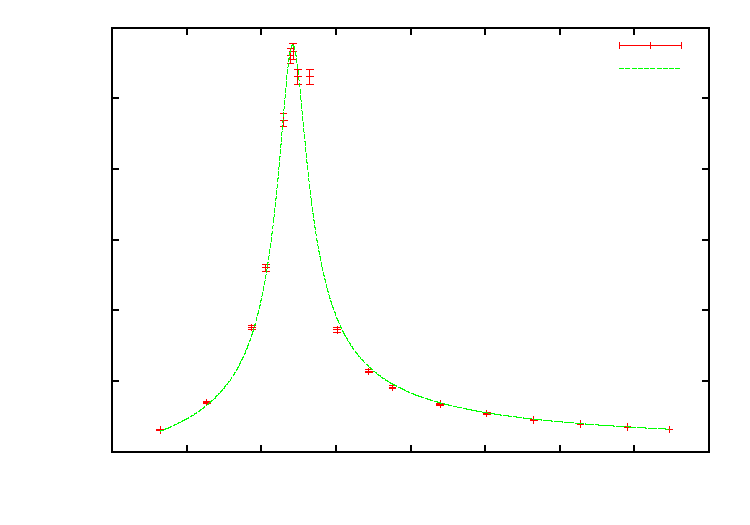
\includegraphics{messung3}}%
    \gplfronttext
  \end{picture}%
\endgroup

	\caption{Scheinwiderstand des Parallelkreises als Funktion der Kreisfrequenz.}
	\label{fig:messung3}
\end{figure}

\section{Diskussion}
\label{sec:diskussion}
\renewcommand{\arraystretch}{1.4} 
\begin{table}
\centering
\begin{tabular}{|c|c|}
\hline
Messgröße		&	Gewichteter Mittelwert\\\hline\hline
$\overline{\omega_R}$	&	$(1199.9\pm 2.3)\,\si{\hertz}$\\\hline
$\overline R$		&	$(80.3 \pm 0.5)\,\si{\ohm}$\\\hline
$\overline L$		&	$(386.2 \pm 0.6)\,\si{\milli\henry}$\\\hline
$\overline C$		&	$(1.800 \pm 0.005)\,\si{\micro\farad}$\\\hline
\end{tabular}
\caption{Mittelwerte aus allen Messungen}
\label{tab:mittelwerteserie}
\end{table}

\subsection{Serienschaltung}
In Abb. \ref{fig:messung3} ist zu erkennen, dass der 2. aufgezeichnete Wert deutlich von der Theoriekurve abweicht, obwohl die anderen relativ dicht an ihr liegen.
Schon während der Messung stach dieser Wert aus den anderen heraus.
Dies könnte daran liegen, dass das Oszilloskop statt $-107\si\degree\quad +107\si\degree$ angezeigt hat, was $-73\si\degree$ entspräche und gut in die Kurve passte.\\

Die graphische Auswertung der Teilspannungen aus Abb. \ref{fig:zeigerU} liefert eine Phasenverschiebung von $\varphi=1.396\,$rad, was von dem theoretischen Wert von $\varphi=(1.399 \pm 0.001)\,\si{rad}$ um $3\permil$ abweicht.
Der Wert liegt zwar nicht im Fehlerintervall, aber dies könnte auch an einer falschen graphischen Darstellung liegen.\\

Die Messwerte außer der Resonanzfrequenz (siehe Abschnitt \ref{sec:resodisku}) zeigten zwar größere Streuungen um die Mittelwerte, aber ihre Fehlerintervalle überschneiden sich.



\subsection{Resonanzfrequenz}
\label{sec:resodisku}
Aus allen Messungen sticht die der Resonanzfrequenz positiv heraus.
Die Werte für die Resonanzfrequenz $\omega_R$ waren durchgehend auffallend konsistent und wichen von dem gewichteten Mittelwert von $\overline{\omega_R}=(1199.9\pm2.3)\,\si\hertz$ um höchstens $2\,\si\hertz$ ab.
Dies ist insofern bemerkenswert, als dass die Fehlerintervalle bis zu 10\% des Messwertes ausmachten.
Es spricht dafür, dass keine der Messungen einen systematischen Fehler diesbezüglich aufweist.

\subsection{Parallelschaltung}
Da mit der Parallelschaltung nur einen Versuch durchgefürt wurde, sind keine Vergleiche möglich.
Allerdings 

\subsection{angenommene Fehler}
Die Fehler der Widerstandsmessungen wurden mit $0.1\si\ohm$ abgeschätzt, da das Messgerät diese Genauigkeit bereitstellte.
Die Frequenzmessungen wurden als präzise eingestuft, da hier die kleinsten Fehler zu erwarten waren und somit die anderen Messungen im Verhältnis deutlich unpräziser sind.
Bei den Spannungsmessungen wurden Fehlerintervalle von $0.01\,\si\volt$ angenommen, was die Genauigkeit der Messgeräte von $(0.25\%+1\,\text{Digit})$ nach oben abschätzt.
Ebenso wurde die Strommessung mit $\sigma_I=2\%$ abgeschätzt, was höher als die eigentliche Genauigkeit von $(1\%+1\,\text{Digit})$ ist.


\bibliography{literatur}
\bibliographystyle{babalpha}
\end{document}
